\documentclass{article}
\usepackage[utf8]{inputenc}
\usepackage{amsmath}
\usepackage{amssymb}
\usepackage{graphicx}


\title{1-10 NumCS}
\author{Aaron Zeller}
\date{January 2023}

\begin{document}
\section*{Approximating the Hyperbolic Sine}
We are given the following code that implements a function that evaluates $\sinh$ at a point $x$ using the formula
\begin{equation*}
\sinh\left(x\right) = \frac{e^{x}-e^{-x}}{2}
\end{equation*}

\begin{figure}[!hbt]
    \centering
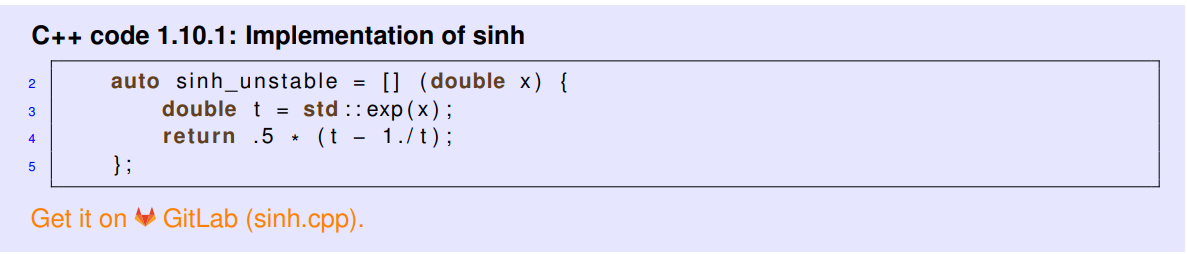
\includegraphics[width=1.0\linewidth]{1-10Code.png}

\end{figure}
\subsection*{1-10.a}
We are tasked with explaining why the code above may not give a good approximation of the hyperbolic sine for small values of $x$, and then compute the relative error using
\begin{equation*}
    \epsilon_{\text{rel}} := \frac{\left
    \lvert \mathrm{sinh\_unstable}\left(x\right) - \sinh\left(x\right)\right\rvert}{\sinh\left(x\right)}
\end{equation*}
with $x = 10^{-k}$, $k = 1,2, \dots, 10$ and implement a \verb|C++| function that computes these results. The problem with the computation lies in us subtracting numbers which are almost the same in the nominator, because $e^{x} \approx e^{-x}$ for $x$ close to zero, hence cancellation occurs. This produces the following code
\begin{figure}[!hbt]
    \centering
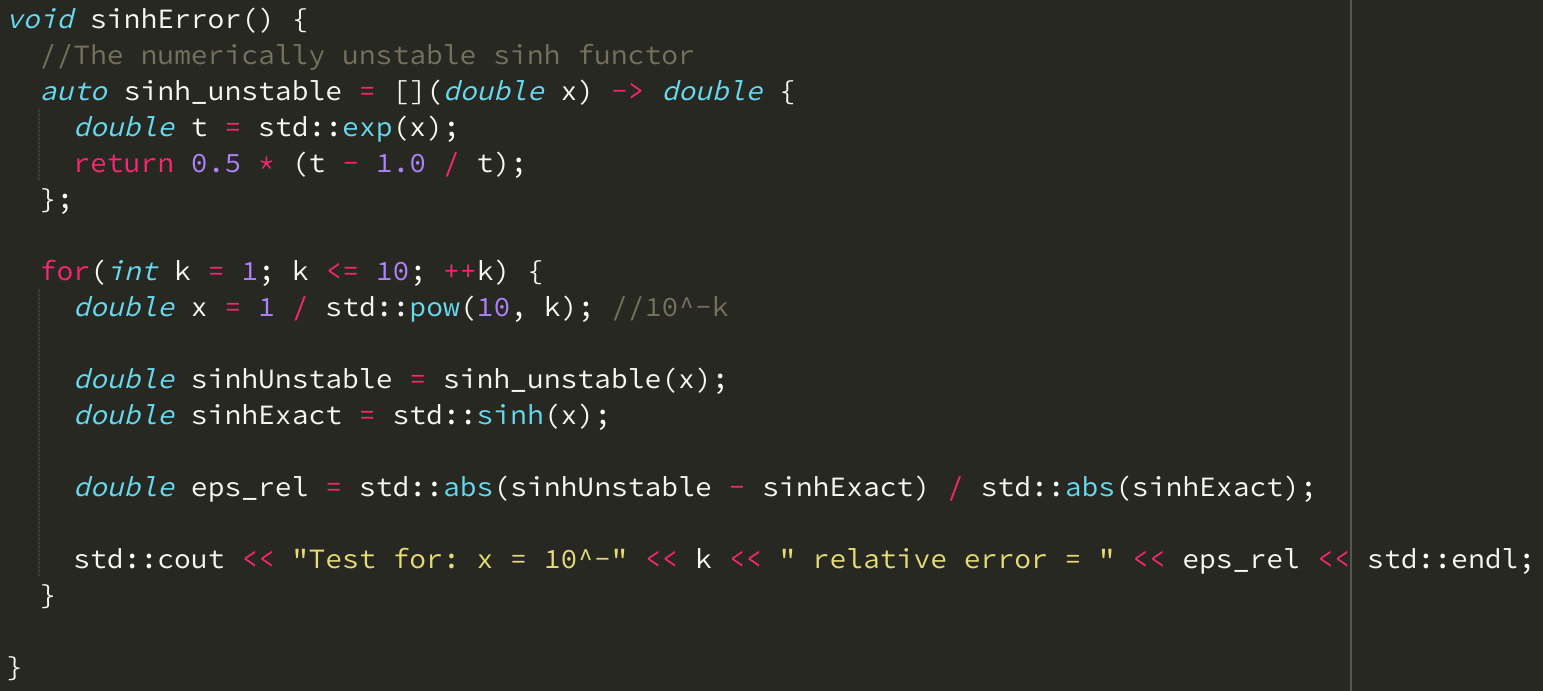
\includegraphics[width=1.0\linewidth]{SinhError1-10.png}
\end{figure}

\pagebreak

\noindent giving us the following output

\begin{figure}[!hbt]
    \centering
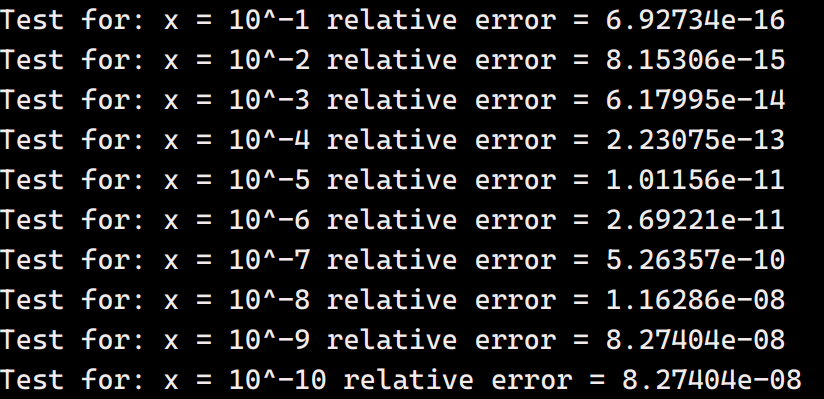
\includegraphics[width=0.7\linewidth]{ErrorOutput1-10.png}
\end{figure}
\subsection*{1-10.b}
We are tasked with writing down the Taylor expansion with $m$ terms around $x=0$ of the function $x \mapsto e^{x}$ and use the same remainder term expression as in 1.5.4.26. The Taylor expansion will be of the form
\begin{equation*}
    f\left(x_{0} + h\right) = \sum_{k=0}^{m}\frac{1}{k!}f^{\left(k\right)}\left(x_{0}\right)h^{k} + \mathrm{R}_{m}\left(x_{0},h\right)\,,\quad \mathrm{R}_{m}\left(x_{0}, h\right) = \frac{1}{\left(m+1\right)!}f^{\left(m+1\right)}\left(\zeta\right)h^{m+1}
\end{equation*}
the exponential function has the following Taylor expansion at $x_{0} = 0$ (hence $f\left(x_{0} + h\right) = f\left(h\right)$ and we have $\left(e^{x}\right)^{\left(k\right)} = e^{x}$ for any $k \in \mathbb{N}^{+}$)
\begin{align*}
    \exp\left(h\right) = \sum_{k=0}^{m}\frac{1}{k!}\text{exp}^{\left(k\right)}\left(0\right)h^{k} + \mathrm{R}_{m}\left(0,h\right) &= \sum_{k=0}^{m}\frac{1}{k!}h^{k} + \mathrm{R}_{m}\left(0,h\right) \\
    &= \sum_{k=0}^{m}\frac{h^{k}}{k!} + \mathrm{R}_{m}\left(0,h\right)
\end{align*}
we then have for $\zeta_{x} \in \left[0,x\right]$
\begin{equation*}
    \mathrm{R}_{m}\left(0,h\right) = \frac{1}{\left(m+1\right)!}\text{exp}^{\left(m+1\right)}\left(\zeta_{x}\right)h^{m+1} = \frac{e^{\zeta_{x}}h^{m+1}}{\left(m+1\right)!}
\end{equation*}
expressed with $x=h$ instead to be consistent with the master solution we get
\begin{equation*}
    e^{x} = \sum_{k=0}^{m}\frac{x^{k}}{k!} + \frac{e^{\zeta_{x}}x^{m+1}}{\left(m+1\right)!} \,,\quad \zeta_{x} \in \left[0,x\right]
\end{equation*}
\subsection*{1-10.c}
We are tasked with proving that for every $x \geq 0$ the following inequality holds true
\begin{equation*}
    \text{sinh}\left(x\right) \geq x \quad \forall\,x \geq 0
\end{equation*}
we then use the definition of $\sinh$
\begin{equation*}
    \sinh\left(x\right) = \frac{e^{x}-e^{-x}}{2}
\end{equation*}
which then gives us
\begin{equation*}
    \sinh\left(x\right) \geq x \Longleftrightarrow \frac{e^{x}-e^{-x}}{2} \geq x \Longleftrightarrow e^{x}-e^{-x} \geq 2x \Longleftrightarrow e^{x} - e^{-x} - 2 \geq 0
\end{equation*}
for $x \geq 0$ we have $e^{x} \geq 1$ and as a consequence $e^{-x} \leq 1$, we have that $e^{x}$ is strictly monotonically increasing and $e^{-x}$ is strictly monotonically decreasing, hence the term
\begin{equation*}
    e^{x} - e^{-x}
\end{equation*}
itself is strictly monotonically increasing, hence because for $x = 0$ we get
\begin{equation*}
    e^{0}-e^{-0} - 2 \cdot 0 = 1 - 1 - 0 = 0 \geq 0
\end{equation*}
and because $e^{x} - e^{-x}$ grows faster than $2x$ ($\left(e^{x}-e^{-x} -2x\right)' = e^{x} + e^{-x} -2 \geq 0$) we can conclude that we always must have 
\begin{equation*}
    e^{x} - e^{-x} - 2 \geq 0
\end{equation*}
and hence as a consequence
\begin{equation*}
    \sinh\left(x\right) \geq x \quad \forall\, x \geq 0
\end{equation*}
\subsection*{1-10.d}
We are tasked with using the Taylor expansion to avoid cancellation by approximating $\sinh\left(x\right)$ for every $0 \leq x \leq 10^{-3}$ such that the relative error $\epsilon_{\text{rel}}$ is smaller than $10^{-15}$. We have that
\begin{equation*}
    \sinh\left(x\right) = \frac{e^{x}-e^{-x}}{2} = \frac{1}{2}\sum_{k=0}^{m}\left(1- \left(-1\right)^{k}\right)\frac{x^{k}}{k!} + \frac{e^{\zeta_{x}}x^{m+1} + e^{\zeta_{-x}}\left(-x\right)^{m+1}}{2\left(m+1\right)!}
\end{equation*}
We can see that if $m \to \infty$ then the denominator $2\left(m+1\right) \to 0$ and hence the remainder term is what we will use to determine the relative error. We consider the approximation given by removing the remainder
\begin{equation*}
    y_{m}\left(x\right) = \frac{1}{2}\sum_{k=0}^{m}\left(1- \left(-1\right)^{k}\right)\frac{x^{k}}{k!}  
\end{equation*} 
the error is now given by the remainder, i.e.
\begin{equation*}
    y_{m}\left(x\right) - \sinh\left(x\right) = \frac{e^{\zeta_{x}}x^{m+1} + e^{\zeta_{-x}}\left(-x\right)^{m+1}}{2\left(m+1\right)!} = \frac{\left(e^{\zeta_{x}} - e^{\zeta_{-x}}\right)x^{m+1}}{2\left(m+1\right)!}
\end{equation*}

\pagebreak

\noindent We now have $0 \leq e^{\zeta_{-x}} \leq e^{x} \leq e^{\zeta_{x}}$ and thus the relative error can be bounded by
\begin{equation*}
    \epsilon_{n, \text{rel}} := \frac{\left\lvert y_{n} - \sinh\left(x\right)\right\rvert}{\sinh\left(x\right)}  = \frac{\left\lvert \frac{\left(e^{\zeta_{x}} - e^{\zeta_{-x}}\right)x^{m+1}}{2\left(m+1\right)!}\right\rvert}{\sinh\left(x\right)} \leq \frac{\left\lvert \frac{\left(0 - e^{x}\right)x^{m+1}}{2\left(m+1\right)!}\right\rvert}{\sinh\left(x\right)} \overset{\substack{0\leq x \leq 10^{-3} \\[0.5mm] 0 \leq \sinh\left(x\right) \leq 1}}{\leq} \left\lvert \frac{\left(-e^{x}\right)x^{m+1}}{2\left(m+1\right)!}\right\rvert =  \frac{e^{x}x^{m+1}}{2\left(m+1\right)!}
\end{equation*}
hence we have 
\begin{equation*}
    \epsilon_{n, \text{rel}} \leq \frac{e^{x}x^{m+1}}{2\left(m+1\right)!}
\end{equation*}
for $m = 3$ we hence get for $x=10^{-3}$ (thr furthest away from $x_{0} = 0$)
\begin{equation*}
    \frac{e^{10^{-3}}\left(10^{-3}\right)^{3+1}}{2\left(3+1\right)!} \approx 2.085 \cdot 10^{-14}
\end{equation*}
and for $m=4$ we get 
\begin{equation*}
    \frac{e^{10^{-3}}\left(10^{-3}\right)^{4+1}}{2\left(4+1\right)!} \approx 4.171\cdot 10^{-18}
\end{equation*}
hence $y_{4}\left(x\right)$ gives already a relative error below $10^{-15}$ as requires by the exercise description.

\end{document}
